\documentclass[11pt,a4paper]{article}

% ---------- Paquetes ----------
\usepackage[utf8]{inputenc}
\usepackage[T1]{fontenc}
\usepackage[spanish]{babel}
\usepackage[margin=2.5cm]{geometry}
\usepackage{graphicx}
\usepackage{booktabs}
\usepackage{array}
\usepackage{tabularx}
\usepackage{longtable}
\usepackage{xcolor}
\usepackage{caption}
\usepackage{enumitem}
\usepackage{amsmath}
\usepackage{textcomp}
\usepackage[colorlinks=true,linkcolor=blue!50!black,citecolor=blue!50!black,urlcolor=blue!50!black]{hyperref}
\usepackage{fancyhdr}
\usepackage{titlesec}

\pagestyle{fancy}
\fancyhf{}
\fancyhead[L]{\small Privacidad Diferencial en Campañas Bancarias}
\fancyhead[R]{\small DS3031 --- Ética y Seguridad de Datos}
\fancyfoot[C]{\thepage}
\renewcommand{\headrulewidth}{0.4pt}

\titleformat{\section}{\normalfont\Large\bfseries}{\thesection.}{0.6em}{}
\titleformat{\subsection}{\normalfont\large\bfseries}{\thesubsection.}{0.6em}{}
\titleformat{\subsubsection}{\normalfont\normalsize\bfseries}{\thesubsubsection.}{0.6em}{}

% Hanging-indent bibliography items (estilo APA, sin paquete adicional)
\newcommand{\refitem}[1]{\par\noindent\hangindent=1.2em\hangafter=1 #1\par\smallskip}

\newcommand{\eps}{\ensuremath{\varepsilon}}

\begin{document}

\renewcommand{\tablename}{Cuadro}
\renewcommand{\figurename}{Figura}

% =====================================================================
% PORTADA
% =====================================================================
\begin{titlepage}
\centering
\vspace*{1.5cm}
{\large Universidad de Ingeniería y Tecnología --- UTEC\par}
{\large DS3031 --- Ética y Seguridad de los Datos\par}
\vspace{1.2cm}
{\Large\bfseries Proyecto Final\par}
\vspace{0.4cm}
{\Large\bfseries Sistema Seguro de Apoyo a Campañas Bancarias\par}
{\Large\bfseries con Privacidad Diferencial\par}
\vspace{1.6cm}
{\large Seguridad de la información y privacidad diferencial como capas complementarias:\par}
{\large una DPIA, un notebook reproducible y un dashboard interactivo\par}
{\large sobre el Bank Marketing Dataset\par}
\vspace{2cm}

\begin{tabular}{ll}
\textbf{Profesor:} & Pazos Ortiz, Jose Carlos \\[0.3cm]
\textbf{Estudiantes} & \textbf{Código} \\
Mora Huamanchay, Angel Obed & 202010031 \\
Surco Vergara, Maria Fernanda & 202110358 \\
Villarreal Falcon, Mishelle Stephany & 202010177 \\
\end{tabular}

\vfill
{\large \today\par}
\end{titlepage}

\tableofcontents
\newpage

% =====================================================================
\section{Introducción}
% =====================================================================

Este proyecto diseña e implementa un sistema seguro de apoyo a campañas bancarias sobre el
\textbf{Bank Marketing Dataset} (Moro et al., 2014), con dos capas de protección que se
complementan y refuerzan mutuamente. La primera es la \textbf{seguridad de la información}:
cifrado AES-256-GCM de datos personales, hashing Argon2id de contraseñas, control de acceso
basado en roles (RBAC) y registros de auditoría, que responden a la pregunta \emph{``¿quién puede
acceder a qué dato, y queda registro de ello?''}. La segunda es la \textbf{privacidad
diferencial}, que responde una pregunta distinta pero igual de importante: \textbf{¿qué se puede
inferir sobre un cliente incluso cuando nadie accede directamente a la base de datos, sino solo a
un reporte agregado o a un modelo entrenado sobre ella?}

Un sistema que solo controla el acceso directo a sus registros, pero publica reportes agregados o
modelos predictivos sin ninguna protección adicional, deja una superficie de riesgo entera sin
cubrir: un atacante no necesita robar la base de datos si puede reconstruir información sensible a
partir de estadísticas ``inocuas'' o de las predicciones de un modelo entrenado sobre datos
reales. Por eso este proyecto integra, desde el diseño, ambas capas: control de accesos y cifrado
para el dato en reposo y en tránsito, y \textbf{privacidad diferencial (DP)} —con la librería
\textbf{IBM diffprivlib} (Holohan et al., 2019)— para todo lo que el sistema libera como
estadística agregada o como salida de un modelo de priorización de clientes.

Este informe, junto con el notebook \texttt{notebooks/01\_privacidad\_diferencial.ipynb} y el
dashboard interactivo (\texttt{frontend/}, respaldado por endpoints FastAPI en
\texttt{backend/app/dp/}) que lo sustentan, documenta el sistema completo. El documento está
organizado en cuatro bloques. Primero, el \textbf{marco legal y normativo} que rige el
tratamiento de datos personales en este proyecto. Segundo, una \textbf{DPIA formal} (Evaluación
de Impacto en la Protección de Datos) que identifica y evalúa los riesgos específicos de este
tratamiento bajo la normativa peruana vigente. Tercero, la \textbf{metodología y los resultados
experimentales} de aplicar DP sobre \texttt{bank.csv}: cuánto ruido hace falta, cuánta utilidad se
pierde, y qué pasa con la equidad del sistema. Cuarto, una \textbf{reflexión ética} que conecta
estos hallazgos con los casos discutidos en el curso (Gender Shades, COMPAS, Toeslagenaffaire, el
teorema de imposibilidad de Kleinberg) y con las decisiones concretas de diseño tomadas en este
sistema.

% =====================================================================
\section{Marco legal y normativo aplicable}
% =====================================================================

El tratamiento de datos personales de este proyecto se enmarca en la normativa peruana de
protección de datos, complementada por estándares internacionales reconocidos. Esta sección
presenta los instrumentos aplicables y su relación con las decisiones de diseño del sistema,
tanto en su capa de seguridad como en su capa de privacidad diferencial.

\subsection{Ley N.\textdegree{} 29733 --- Ley de Protección de Datos Personales}

Promulgada en 2011, es el marco legal peruano principal para el tratamiento de datos personales,
y da desarrollo al derecho fundamental reconocido en el artículo 2, numeral 6, de la Constitución
Política del Perú. Su reglamento vigente es el \textbf{Decreto Supremo N.\textdegree{}
016-2024-JUS} (30 de noviembre de 2024, en vigor desde el 29 de marzo de 2025), que actualizó el
marco peruano alineándolo con el RGPD europeo y con ISO/IEC 27001, ampliando la definición de
datos personales y reforzando los principios de \textbf{privacidad por diseño y por defecto} y de
\textbf{responsabilidad proactiva (accountability)}.

Los principios rectores de la Ley N.\textdegree{} 29733 más relevantes para el diseño de este
sistema son:

\begin{table}[htbp]
\centering
\small
\begin{tabularx}{\textwidth}{@{}p{3.2cm}X@{}}
\toprule
\textbf{Principio} & \textbf{Aplicación en el sistema} \\
\midrule
Proporcionalidad &
Un reporte agregado (media de saldo, conteo de clientes por campaña) no necesita revelar el valor
exacto para cumplir su finalidad de negocio --- un valor con ruido calibrado es proporcional al
fin perseguido. \\
\addlinespace
Privacidad por diseño y por defecto (D.S. 016-2024-JUS) &
La incorporación de DP en la capa de reportes y modelos, junto con el cifrado y el control de
accesos en la capa de datos, instancia técnicamente este principio: la protección se construye en
el mecanismo de cómputo y de acceso mismos, no se añade después. \\
\addlinespace
Minimización de datos &
Los identificadores directos nunca participan en reportes ni en el modelo, y el modelo con DP
nunca ``ve'' el dato exacto de un cliente individual con una influencia no acotada --- el
mecanismo de perturbación objetivo limita estructuralmente cuánto puede depender la salida de un
solo registro. \\
\addlinespace
Seguridad &
Cifrado AES-256-GCM en reposo, TLS en tránsito, hashing Argon2id de contraseñas, control de
accesos basado en roles (RBAC) y registros de auditoría sobre todo acceso a datos sensibles. \\
\bottomrule
\end{tabularx}
\caption{Principios de la Ley N.\textdegree{} 29733 aplicados al sistema.}
\end{table}

La ANPDP (Autoridad Nacional de Protección de Datos Personales, dependiente del MINJUS) es el
órgano supervisor; el plan de respuesta a incidentes del sistema contempla su notificación en
caso de fuga, tanto si ocurre por una brecha directa a la base de datos como si ocurre por
reportes agregados indebidamente precisos.

\subsection{Estándares internacionales}

El diseño del sistema toma como referencia \textbf{ISO/IEC 27001} (SGSI), \textbf{ISO/IEC 27701}
(extensión de privacidad), \textbf{NIST SP 800-53} y \textbf{NIST SP 800-61} (controles de
seguridad y respuesta a incidentes), \textbf{OWASP Top 10}, y, específicamente para la capa de
privacidad diferencial, el marco de \textbf{NIST SP 800-226}, \emph{Guidelines for Evaluating
Differential Privacy Guarantees} (borrador de NIST sobre buenas prácticas para desplegar DP en
producción), que orienta la elección de \eps{} y la documentación de supuestos (como el
\texttt{data\_norm} discutido en la Sección 5.3) como parte de la debida diligencia técnica
exigible bajo el principio de responsabilidad proactiva.

\subsection{Consentimiento y privacidad diferencial: un matiz importante}

El sistema gestiona el consentimiento del cliente mediante los estados \texttt{opt-in} /
\texttt{opt-out} / \texttt{no informado}. Sin embargo, ese consentimiento cubre \textbf{si el
cliente puede ser contactado}, no \textbf{cuánto ruido de privacidad se aplica cuando su registro
entra a un reporte agregado o a un modelo}. Esta es una limitación estructural que se discute en
la Sección 7.3: el marco de consentimiento binario del sistema no tiene un mecanismo para que un
cliente exprese preferencias sobre su ``presupuesto de privacidad'' individual, algo que excede el
alcance de la Ley N.\textdegree{} 29733 pero que la literatura de DP local (Apple, 2017) sí
contempla como posibilidad de diseño futuro.

% =====================================================================
\section{Caso de negocio y dataset}
% =====================================================================

Una entidad bancaria busca priorizar clientes para campañas de depósito a plazo, balanceando el
valor comercial (KPIs de conversión, costo de adquisición, reducción de llamadas no efectivas) con
la protección de la información de sus clientes. El sistema aborda esa tensión desde dos frentes
que operan en conjunto: controlar \textbf{quién accede} a la base de datos, y controlar
\textbf{cuánta información revela} cualquier reporte o modelo que se derive de ella.

El dataset base es \texttt{bank.csv}, 11\,162 registros, 17 atributos, sin valores nulos,
derivado de Moro, Cortez y Rita (2014) vía Kaggle (Bachmann, 2018). Sus columnas se clasifican en
cuatro cuasi-identificadores demográficos (\texttt{age}, \texttt{job}, \texttt{marital},
\texttt{education}) y cinco atributos sensibles financieros/de comportamiento (\texttt{balance},
\texttt{default}, \texttt{housing}, \texttt{loan}, \texttt{deposit}). Esta clasificación es la
base directa del análisis de riesgo de la DPIA (Sección 4) y del notebook técnico. El sistema
complementa este dataset con datos sintéticos (identificadores de cliente, contacto, usuarios
internos, roles y registros de auditoría, generados con Faker y semilla fija) para representar un
entorno bancario realista sobre el cual operan tanto los controles de seguridad como la capa de
privacidad diferencial.

% =====================================================================
\section{Evaluación de Impacto en la Protección de Datos (DPIA)}
% =====================================================================

\subsection{Descripción del tratamiento y finalidad}

\begin{table}[htbp]
\centering
\small
\begin{tabularx}{\textwidth}{@{}p{3.6cm}X@{}}
\toprule
\textbf{Campo} & \textbf{Descripción} \\
\midrule
Responsable del tratamiento &
Entidad bancaria (simulada), a través del área de Marketing con soporte del área de Data y
Gobernanza. \\
\addlinespace
Finalidad del tratamiento &
(a) Priorizar clientes elegibles para campañas de depósito a plazo según un modelo de
propensión; (b) generar reportes agregados de desempeño de campaña (saldo promedio, distribución
demográfica de clientes contactados) para supervisión y cumplimiento de KPIs/OKRs. \\
\addlinespace
Base de licitud &
Consentimiento del titular (estado \texttt{opt-in} en la tabla \texttt{consentimiento}) para el
contacto comercial; interés legítimo del responsable para el análisis agregado con fines de
mejora del servicio, sujeto a las medidas de minimización descritas abajo. \\
\addlinespace
Categorías de titulares &
Clientes actuales o potenciales de productos bancarios (personas naturales). \\
\addlinespace
Alcance del tratamiento &
Comprende tanto el acceso directo a registros individuales (controlado por RBAC) como la
\textbf{publicación de agregados y de un modelo predictivo}, que constituye una superficie de
tratamiento adicional evaluada específicamente en esta DPIA. \\
\bottomrule
\end{tabularx}
\caption{Descripción del tratamiento y su finalidad.}
\end{table}

\subsection{Inventario y clasificación de datos personales}

\begin{table}[htbp]
\centering
\scriptsize
\begin{tabularx}{\textwidth}{@{}p{3cm}p{2.6cm}XX@{}}
\toprule
\textbf{Dato} & \textbf{Clasificación} & \textbf{Tratamiento (capa de seguridad)} &
\textbf{Tratamiento (capa de privacidad diferencial)} \\
\midrule
\texttt{nombre}, \texttt{dni}, \texttt{email}, \texttt{telefono}, \texttt{direccion} (sintéticos)
& Dato personal identificable &
Cifrado AES-256-GCM en reposo &
No participan en reportes agregados ni en el modelo --- excluidos por diseño (minimización) \\
\addlinespace
\texttt{age}, \texttt{job}, \texttt{marital}, \texttt{education} & Dato personal
(cuasi-identificador) &
Acceso restringido por rol &
Sujeto a DP en histogramas/conteos; usado como feature del modelo con DP \\
\addlinespace
\texttt{balance}, \texttt{default}, \texttt{housing}, \texttt{loan} & Dato financiero &
Acceso limitado por rol &
Sujeto a DP en consultas agregadas (media de \texttt{balance}); features del modelo con DP \\
\addlinespace
\texttt{deposit} & Variable objetivo / dato de comportamiento & --- &
Variable predicha por el modelo; su distribución agregada también se protege con DP en reportes \\
\addlinespace
Estado de \texttt{consentimiento} & Dato de privacidad &
Trazabilidad de cambios, bloqueo de campañas si opt-out &
No se altera; sigue gobernando exclusivamente la elegibilidad de contacto (ver limitación en
\S2.3) \\
\bottomrule
\end{tabularx}
\caption{Inventario y clasificación de datos personales.}
\end{table}

\subsection{Identificación de riesgos}

\begin{enumerate}[leftmargin=1.4em]
\item \textbf{Reidentificación por cuasi-identificadores.} Medido empíricamente en la Sección 6.1:
$\sim$8\% de los registros son únicos ($k=1$) usando solo 4 atributos demográficos. Un atacante
con acceso a un reporte que cruce estos atributos con un atributo sensible podría reidentificar a
una fracción no trivial de clientes.
\item \textbf{Inferencia de pertenencia (\emph{membership inference}) sobre el modelo publicado.}
Si el modelo de propensión se expone (p.\,ej. como servicio de \emph{scoring}, o si sus
parámetros se comparten con un proveedor externo), un atacante puede, en principio, inferir si un
individuo específico formó parte del conjunto de entrenamiento, explotando el sobreajuste del
modelo a esos registros.
\item \textbf{Discriminación algorítmica.} El modelo baseline (sin ninguna protección de
privacidad) ya exhibe una brecha de paridad demográfica de 0.077 entre grupos etarios (Sección
6.2) --- si ese modelo se usa para decidir a quién priorizar, el sesgo se traduce directamente en
una práctica comercial potencialmente discriminatoria y en un riesgo regulatorio bajo el
principio de proporcionalidad de la Ley N.\textdegree{} 29733.
\item \textbf{Reversión/extracción de atributos sensibles desde reportes agregados de alta
precisión.} Publicar una media de \texttt{balance} exacta por segmento demográfico pequeño (p.\,ej.
``mujeres solteras, 18-25 años, en la sucursal X'') puede, combinada con otras fuentes, acercarse
peligrosamente a revelar el valor individual cuando el segmento es muy pequeño (conecta
directamente con el hallazgo de k-anonimato de la Sección 6.1).
\item \textbf{Fuga de datos por brecha en la base de datos.} Mitigado mediante cifrado
AES-256-GCM, TLS, RBAC y auditoría; se mantiene como riesgo de fondo, evaluado también respecto a
si una brecha expondría los parámetros del modelo entrenado sin DP (que memorizan más información
de los datos de entrenamiento que un modelo entrenado con DP).
\end{enumerate}

\subsection{Matriz de probabilidad $\times$ impacto}

\begin{table}[htbp]
\centering
\small
\begin{tabularx}{\textwidth}{@{}p{3.6cm}p{2cm}p{1.6cm}p{2.4cm}X@{}}
\toprule
\textbf{Riesgo} & \textbf{Prob.\ (sin mitigación)} & \textbf{Impacto} & \textbf{Nivel (sin
mitigación)} & \textbf{Nivel (con mitigación completa)} \\
\midrule
Reidentificación por cuasi-identificadores en reportes agregados & Alta & Alto & \textbf{Crítico}
& Bajo \\
Inferencia de pertenencia sobre el modelo & Media & Medio & \textbf{Medio} & Bajo-Medio \\
Discriminación algorítmica en priorización de campañas & Alta & Alto & \textbf{Crítico} & Medio
\emph{(DP no la elimina --- ver \S4.5 y \S6.5)} \\
Reversión de atributos sensibles vía agregados de segmentos pequeños & Alta & Alto &
\textbf{Crítico} & Bajo \\
Fuga de datos por brecha en la BD (parámetros del modelo incluidos) & Baja \emph{(post-controles
de seguridad)} & Crítico & \textbf{Medio} & Medio-Bajo \emph{(DP reduce cuánto memoriza el
modelo, no elimina el riesgo de brecha en sí)} \\
\bottomrule
\end{tabularx}
\caption{Matriz de probabilidad $\times$ impacto, antes y después de mitigación.}
\end{table}

\subsection{Medidas de mitigación}

\begin{itemize}[leftmargin=1.4em]
\item \textbf{Privacidad diferencial en consultas agregadas} (mecanismo de Laplace,
\texttt{diffprivlib.tools}) para toda estadística que se publique fuera del backend con control
de acceso: medias, conteos, histogramas.
\item \textbf{Privacidad diferencial en el modelo predictivo}
(\texttt{diffprivlib.models.LogisticRegression}, perturbación objetiva) cuando el modelo se vaya
a exponer más allá del equipo interno autorizado por RBAC.
\item \textbf{Minimización de datos}: los identificadores directos (nombre, DNI, email, teléfono,
dirección) nunca participan en el pipeline de reportes ni de entrenamiento del modelo --- siguen
cifrados y aislados en la capa de seguridad del sistema.
\item \textbf{Auditoría de fairness previa a cualquier despliegue} (Sección 6.2 y 6.5): medir
paridad demográfica e igualdad de oportunidad como parte del ciclo de vida del modelo, no como un
chequeo opcional.
\item \textbf{Controles de seguridad de base}: cifrado AES-256-GCM, hashing Argon2id, RBAC, TLS,
registros de auditoría, gestión de consentimiento --- primera línea de defensa sobre la que se
apoya toda la capa de privacidad diferencial.
\end{itemize}

\subsection{Riesgo residual}

Incluso con todas las medidas anteriores, persisten riesgos residuales que deben documentarse de
forma transparente:

\begin{itemize}[leftmargin=1.4em]
\item \textbf{La privacidad diferencial no elimina el sesgo de partida del modelo} --- solo lo
desplaza cuantitativamente (Sección 6.5). Un modelo con DP puede seguir siendo inapropiado para
producción si su brecha de equidad residual no es aceptable para la organización.
\item \textbf{El presupuesto de privacidad (\eps) es una decisión de negocio, no puramente
técnica}: un \eps{} demasiado alto (cercano a 10, régimen ``permisivo'') reduce las garantías
formales de privacidad a niveles poco significativos en la práctica, aunque matemáticamente sigan
siendo DP.
\item \textbf{DP protege la salida publicada, no la base de datos subyacente} --- una brecha
directa a PostgreSQL sigue siendo posible y sigue dependiendo enteramente de los controles de
seguridad de base (cifrado, RBAC), que no forman parte del mecanismo de DP.
\item \textbf{Ataques compuestos}: la combinación de múltiples reportes con DP publicados a lo
largo del tiempo puede erosionar la garantía de privacidad acumulada (\emph{composition} de DP) si
no se gestiona un presupuesto de privacidad total por individuo --- este proyecto no implementa un
contador de presupuesto acumulado, lo cual queda como recomendación futura explícita.
\end{itemize}

% =====================================================================
\section{Metodología de privacidad diferencial}
% =====================================================================

\subsection{Justificación de la librería: IBM diffprivlib}

Se usa \textbf{IBM diffprivlib} (Holohan, Braghin, Mac Aonghusa y Levacher, 2019), una librería de
código abierto que implementa los mecanismos canónicos de la teoría de privacidad diferencial
---Laplace, Gaussian, exponencial--- sobre una API compatible con scikit-learn. Esto permite
sustituir directamente \texttt{df.mean()} por \texttt{diffprivlib.tools.mean(...)}, o
\texttt{sklearn.linear\_model.LogisticRegression} por
\texttt{diffprivlib.models.LogisticRegression}, sin rediseñar el pipeline de análisis existente.
Como comparativa, se evaluó también \textbf{OpenDP} (otra librería de referencia, mantenida por
Harvard/Microsoft) para las consultas de conteo; ambas implementan el mismo mecanismo de Laplace
con garantías formales equivalentes --- se optó por diffprivlib como librería primaria por su
cobertura más amplia de modelos de machine learning listos para usar (regresión logística,
árboles, k-means), que es justamente lo que este caso de uso necesita para el modelo de
propensión.

\subsection{Justificación del rango de \texorpdfstring{\eps}{epsilon} evaluado}

El parámetro \eps{} es el \textbf{presupuesto de privacidad}: cuantifica cuánto puede cambiar la
distribución de la salida de un mecanismo si un solo registro se agrega o se remueve del dataset.
No existe un valor ``correcto'' universal, así que se evaluó un rango que cubre desde un régimen
conservador hasta uno cercano a lo usado en despliegues reales:

\begin{table}[htbp]
\centering
\small
\begin{tabularx}{\textwidth}{@{}p{3.4cm}p{4cm}X@{}}
\toprule
\textbf{Referencia} & \textbf{Régimen de \eps{} reportado} & \textbf{Relevancia para este
proyecto} \\
\midrule
Dwork y Roth (2014) & \eps{} ``pequeño, del orden de 0.1'' para garantías fuertes & Extremo
conservador del rango evaluado \\
US Census Bureau (2021) & Presupuesto total $\eps\approx19.61$ repartido entre consultas
jerárquicas del censo 2020 & Referencia de que en producción a gran escala se opera con
presupuestos más altos que el ``ideal de libro de texto'' \\
Apple (2017) & \eps{} por consulta diaria típicamente entre 2 y 16, según el caso de uso de
telemetría & Extremo permisivo del rango evaluado \\
\bottomrule
\end{tabularx}
\caption{Justificación del rango de \eps{} evaluado.}
\end{table}

Por eso el notebook evalúa $\eps \in \{0.1, 0.5, 1.0, 2.0, 5.0, 10.0\}$: desde el extremo
conservador de Dwork y Roth hasta un extremo cercano al régimen permisivo de Apple/Census,
permitiendo mostrar la curva completa del trade-off en vez de comprometerse de antemano con un
único punto.

\subsection{Mecanismos empleados}

\begin{itemize}[leftmargin=1.4em]
\item \textbf{Mecanismo de Laplace} (\texttt{diffprivlib.mechanisms.Laplace},
\texttt{diffprivlib.tools.mean}, \texttt{diffprivlib.tools.histogram}): usado para consultas
agregadas (media de \texttt{balance}, conteos por \texttt{job}/\texttt{marital}, histograma de
\texttt{age}). La sensibilidad global de cada consulta se calcula explícitamente: para una media
acotada, $(\text{máximo} - \text{mínimo}) / n$; para un conteo, sensibilidad 1 (agregar o quitar
un registro cambia el conteo de su categoría en, como máximo, uno).
\item \textbf{Perturbación objetiva} (\emph{objective perturbation}, Chaudhuri, Monteleoni y
Sarwate, 2011), implementada en \texttt{diffprivlib.models.LogisticRegression}: añade ruido
calibrado directamente a la función de pérdida que optimiza el modelo, en vez de al resultado
final. Requiere una cota pública (\texttt{data\_norm}) sobre la norma L2 de cada fila de
features. En este proyecto se fija explícitamente esa cota usando el percentil 95 de las normas
observadas en el conjunto de entrenamiento, documentando abiertamente que en un despliegue real
esa cota debería fijarse a priori con datos históricos o de dominio ---nunca inferirse del propio
batch de datos privados que se va a proteger, porque eso rompería la garantía formal de DP---.
\end{itemize}

% =====================================================================
\section{Resultados experimentales}
% =====================================================================

Resultados completos, código y celdas ejecutadas en
\texttt{notebooks/01\_privacidad\_diferencial.ipynb}. Esta sección resume los hallazgos y embebe
las figuras generadas por el notebook.

\subsection{Riesgo de reidentificación (k-anonimato empírico)}

Sobre los 11\,162 registros de \texttt{bank.csv}, agrupando por los 4 cuasi-identificadores
(\texttt{age}, \texttt{job}, \texttt{marital}, \texttt{education}), se obtuvieron \textbf{2\,293
combinaciones distintas}:

\begin{itemize}[leftmargin=1.4em]
\item \textbf{$k$ mínimo observado: 1} (registros completamente únicos).
\item \textbf{7.99\% de los registros son únicos} ($k=1$) --- reidentificables de forma directa si
un atacante conoce esos 4 atributos de una persona real.
\item \textbf{26.76\% de los registros tienen $k<5$}, y \textbf{43.68\% tienen $k<10$}.
\end{itemize}

\begin{figure}[htbp]
\centering
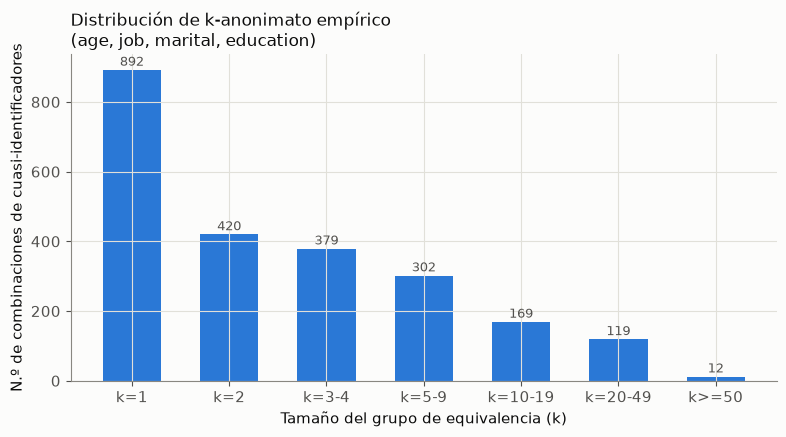
\includegraphics[width=0.85\textwidth]{informe_assets/01_kanonimato.png}
\caption{Distribución de k-anonimato empírico (\texttt{age}, \texttt{job}, \texttt{marital},
\texttt{education}).}
\end{figure}

Esto confirma que remover identificadores directos (como hace la capa de cifrado del sistema
sobre las columnas \texttt{*\_cifrado}) \textbf{no es suficiente} para anonimizar el dataset: el
riesgo de reidentificación vive en la combinación de atributos demográficos aparentemente
inocuos.

\subsection{Baseline sin privacidad diferencial}

Se entrenó un clasificador de referencia (\texttt{LogisticRegression}, sin ningún mecanismo de
privacidad diferencial) para predecir \texttt{deposit}, excluyendo \texttt{duration} por ser una
variable que solo se conoce después de realizar la llamada (fuga de información hacia el futuro,
inutilizable en un escenario real de priorización previa al contacto):

\begin{table}[htbp]
\centering
\begin{tabular}{@{}lc@{}}
\toprule
\textbf{Métrica} & \textbf{Valor} \\
\midrule
Accuracy & 0.6965 \\
F1-score & 0.6366 \\
ROC-AUC & 0.7573 \\
\bottomrule
\end{tabular}
\caption{Métricas del modelo baseline (sin DP).}
\end{table}

\begin{figure}[htbp]
\centering
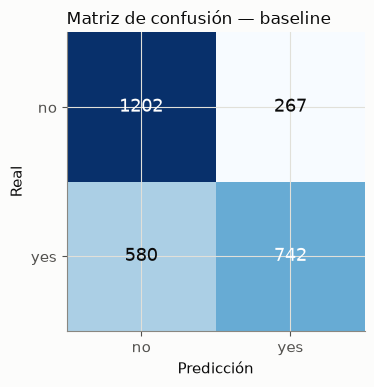
\includegraphics[width=0.55\textwidth]{informe_assets/02_matriz_confusion_baseline.png}
\caption{Matriz de confusión --- baseline.}
\end{figure}

\textbf{Fairness del baseline} (grupo protegido: edad, \texttt{joven <35} vs.\ \texttt{no\_joven
$\geq$35}):

\begin{table}[htbp]
\centering
\begin{tabular}{@{}lccc@{}}
\toprule
\textbf{Grupo} & $n$ & \textbf{P(predicción = ``sí'')} & \textbf{TPR (igualdad de oportunidad)} \\
\midrule
joven ($<$35) & 923 & 0.4128 & 0.5773 \\
no\_joven ($\geq$35) & 1868 & 0.3362 & 0.5526 \\
\bottomrule
\end{tabular}
\caption{Fairness del modelo baseline por grupo etario.}
\end{table}

\begin{itemize}[leftmargin=1.4em]
\item Diferencia de \textbf{paridad demográfica}: \textbf{0.0766}
\item Diferencia de \textbf{igualdad de oportunidad}: \textbf{0.0247}
\end{itemize}

El modelo baseline ya trata a los dos grupos etarios de forma distinta \textbf{antes de introducir
cualquier mecanismo de privacidad} --- un punto de partida importante para interpretar los
resultados de la Sección 6.4.

\subsection{Consultas agregadas con privacidad diferencial}

\textbf{Media de \texttt{balance}} (media real: 1\,528.54 EUR; cota de sensibilidad: rango
completo $[-6\,847,\ 81\,204]$ EUR):

\begin{table}[htbp]
\centering
\begin{tabular}{@{}cc@{}}
\toprule
\textbf{\eps} & \textbf{Error absoluto medio (EUR)} \\
\midrule
0.1 & 75.43 \\
0.5 & 16.68 \\
1.0 & 9.57 \\
2.0 & 2.89 \\
5.0 & 1.98 \\
10.0 & 0.69 \\
\bottomrule
\end{tabular}
\caption{Error de la media de \texttt{balance} con DP, por \eps.}
\end{table}

\textbf{Conteos por categoría} (mecanismo de Laplace, sensibilidad $=1$):

\begin{table}[htbp]
\centering
\begin{tabular}{@{}ccc@{}}
\toprule
\textbf{\eps} & \textbf{Error medio --- conteo \texttt{job}} & \textbf{Error medio --- conteo
\texttt{marital}} \\
\midrule
0.1 & 10.24 & 7.93 \\
0.5 & 2.15 & 2.51 \\
1.0 & 0.98 & 1.22 \\
2.0 & 0.46 & 0.52 \\
5.0 & 0.23 & 0.22 \\
10.0 & 0.10 & 0.11 \\
\bottomrule
\end{tabular}
\caption{Error de conteos con DP, por \eps.}
\end{table}

\begin{figure}[htbp]
\centering
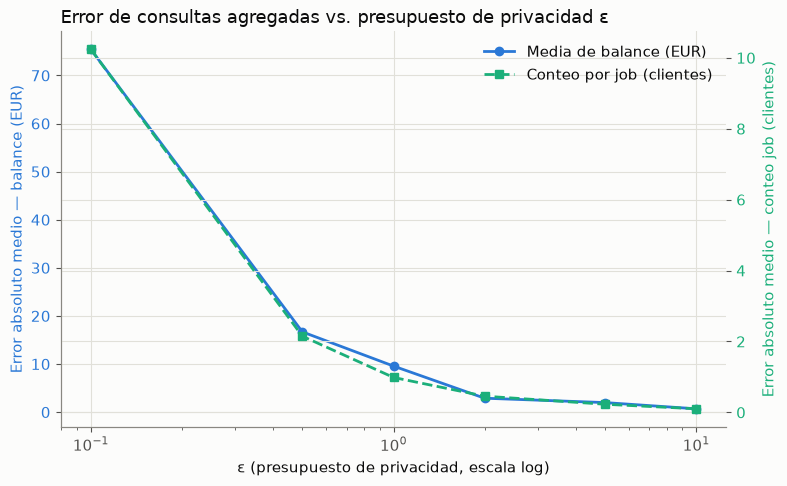
\includegraphics[width=0.85\textwidth]{informe_assets/04_error_vs_epsilon_queries.png}
\caption{Error de consultas agregadas vs. \eps.}
\end{figure}

\begin{figure}[htbp]
\centering
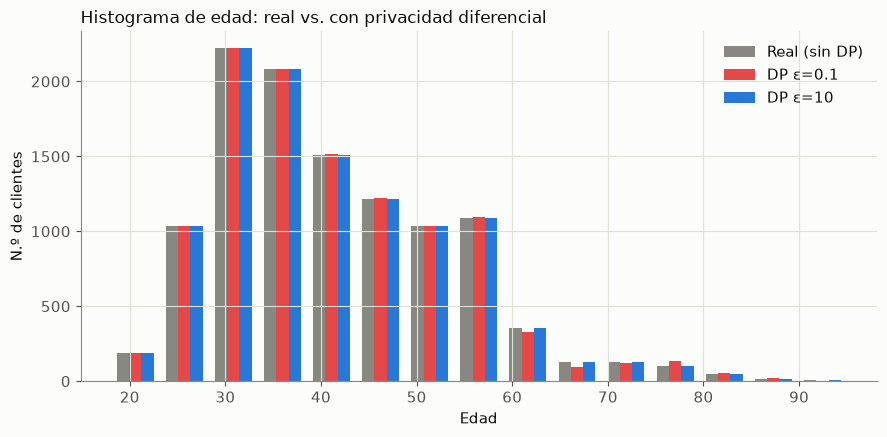
\includegraphics[width=0.85\textwidth]{informe_assets/03_histograma_edad_dp.png}
\caption{Histograma de edad: real vs. con privacidad diferencial.}
\end{figure}

El error de la media de \texttt{balance} es proporcionalmente mucho más sensible a \eps{} bajo que
los conteos, porque el rango de esa columna es muy amplio (de $-6\,847$ a $81\,204$ EUR): a mayor
rango posible de una variable, mayor la sensibilidad global de su media y, por lo tanto, más ruido
de Laplace se necesita para el mismo \eps. Un despliegue real se beneficiaría de acotar
(\emph{clip}) los valores extremos de \texttt{balance} antes de aplicar DP, reduciendo la
sensibilidad a costa de un sesgo controlado en el estimador.

\subsection{Modelo con privacidad diferencial y trade-off privacidad-utilidad}

\begin{table}[htbp]
\centering
\small
\begin{tabular}{@{}cccccc@{}}
\toprule
\textbf{\eps} & \textbf{Accuracy} & \textbf{F1} & \textbf{ROC-AUC} & \multicolumn{2}{c}{\textbf{Pérdida
relativa de F1 vs. baseline}} \\
\midrule
0.1 & 0.5304 & 0.5165 & 0.5410 & \multicolumn{2}{c}{18.87\%} \\
0.5 & 0.5745 & 0.5533 & 0.5996 & \multicolumn{2}{c}{13.10\%} \\
1.0 & 0.5981 & 0.5738 & 0.6247 & \multicolumn{2}{c}{9.87\%} \\
2.0 & 0.5838 & 0.5582 & 0.6001 & \multicolumn{2}{c}{12.33\%} \\
5.0 & 0.6878 & 0.6421 & 0.7389 & \multicolumn{2}{c}{$-0.86\%$ (supera al baseline)} \\
10.0 & 0.6970 & 0.6446 & 0.7529 & \multicolumn{2}{c}{$-1.25\%$ (supera al baseline)} \\
\bottomrule
\end{tabular}
\caption{Modelo con DP vs. baseline (F1 = 0.6366, ROC-AUC = 0.7573).}
\end{table}

\begin{figure}[htbp]
\centering
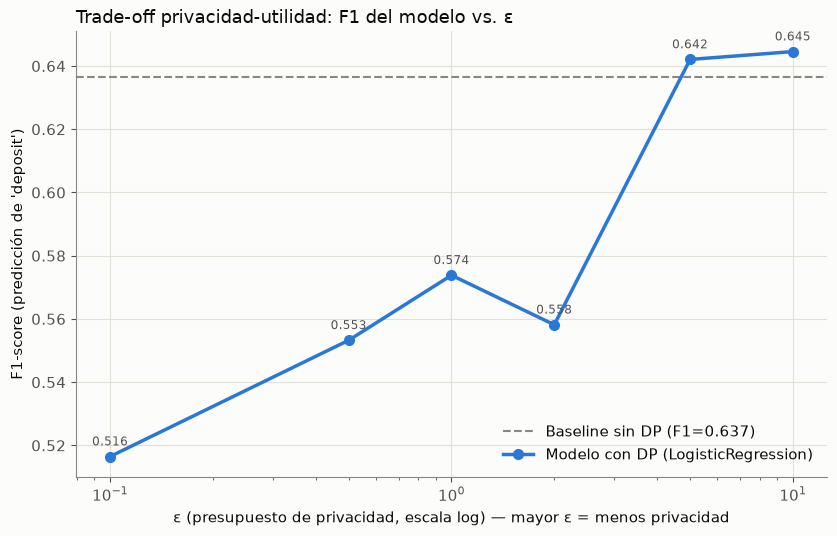
\includegraphics[width=0.85\textwidth]{informe_assets/05_tradeoff_epsilon_f1.png}
\caption{Trade-off privacidad-utilidad: F1 vs. \eps.}
\end{figure}

En el régimen de \eps{} bajo (0.1--0.5) el ruido inyectado en la optimización es tan grande que el
modelo apenas supera una predicción aleatoria (F1$\approx$0.52). La tendencia de fondo al aumentar
\eps{} es claramente positiva, aunque no perfectamente monótona (hay una fluctuación puntual
alrededor de $\eps=2$, esperable porque cada punto es el promedio de un mecanismo aleatorizado).
En $\eps=5$ y $\eps=10$ el modelo con DP \textbf{iguala o incluso supera ligeramente} el F1 y AUC
del baseline --- una particularidad de este dataset y esta corrida (con \texttt{data\_norm} fijado
por percentil, la perturbación objetiva actúa también como una forma leve de regularización), no
una garantía general de que ``DP mejora los modelos''.

\subsection{Fairness bajo privacidad diferencial}

\begin{table}[htbp]
\centering
\begin{tabular}{@{}ccc@{}}
\toprule
\textbf{\eps} & \textbf{Diferencia de paridad demográfica} & \textbf{Diferencia de igualdad de
oportunidad} \\
\midrule
0.1 & 0.1213 & 0.1353 \\
0.5 & 0.0484 & 0.0538 \\
1.0 & 0.0368 & 0.0360 \\
2.0 & 0.0414 & 0.0437 \\
5.0 & 0.0535 & 0.0176 \\
10.0 & 0.0658 & 0.0207 \\
\bottomrule
\end{tabular}
\caption{Fairness bajo DP, por \eps{} (baseline: paridad demográfica $=0.0766$, igualdad de
oportunidad $=0.0247$).}
\end{table}

\begin{figure}[htbp]
\centering
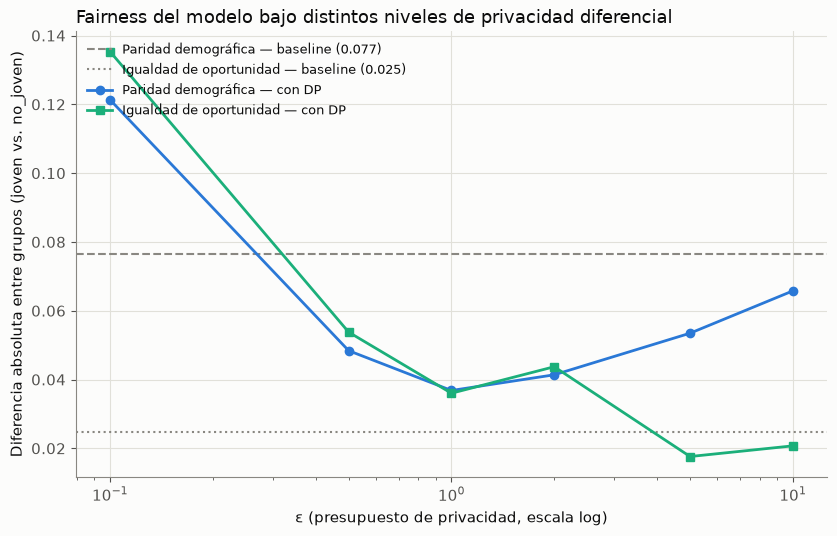
\includegraphics[width=0.85\textwidth]{informe_assets/06_fairness_bajo_dp.png}
\caption{Fairness del modelo bajo distintos niveles de privacidad diferencial.}
\end{figure}

Ambas métricas muestran un pico pronunciado en $\eps=0.1$, muy por encima del baseline --- no
porque el modelo ``aprenda'' a discriminar más, sino porque un clasificador casi aleatorio (por el
exceso de ruido en ese régimen) es inestable estadísticamente entre grupos de tamaño distinto. Lo
más relevante ocurre en el resto del rango evaluado ($\eps\geq0.5$): \textbf{en ningún punto la
brecha del modelo con DP superó a la del baseline sin privacidad}. Este es un resultado empírico
específico de este dataset y este atributo protegido --- no una propiedad garantizada del
mecanismo de DP en general --- y se discute con más profundidad en la Sección 7.4.

% =====================================================================
\section{Reflexión ética}
% =====================================================================

\subsection{Sesgo algorítmico: de Gender Shades y COMPAS a este proyecto}

\textbf{Buolamwini y Gebru (2018)}, en \emph{Gender Shades}, mostraron que los sistemas
comerciales de clasificación de género por imagen facial tenían tasas de error de hasta 34.7
puntos porcentuales más altas para mujeres de piel oscura que para hombres de piel clara --- un
fallo de equidad invisible mientras solo se reportaba la accuracy global del sistema.
\textbf{Angwin, Larson, Mattu y Kirchner (2016)}, en su investigación sobre el sistema COMPAS de
evaluación de riesgo de reincidencia, encontraron que el algoritmo etiquetaba a personas
afroamericanas como de ``alto riesgo'' con una tasa de falsos positivos casi el doble que a
personas blancas.

El paralelismo con este proyecto es directo: el modelo baseline de propensión a depósito también
exhibe una brecha de tratamiento por grupo etario (Sección 6.2) que, de no medirse
explícitamente, habría quedado oculta detrás de una métrica agregada de accuracy o F1 que ``se ve
bien''. La lección metodológica de Gender Shades y COMPAS ---\textbf{reportar métricas
desagregadas por grupo protegido, no solo el desempeño global}--- es exactamente lo que se
implementó en la Sección 6.2 y 6.5 de este trabajo, y debería ser un requisito no negociable antes
de desplegar cualquier modelo de priorización de clientes en producción, con o sin DP.

\subsection{Transparencia}

Uno de los objetivos de diseño del dashboard interactivo de este proyecto es hacer \emph{visible}
el efecto del presupuesto de privacidad mediante un control deslizante de \eps{} que actualiza
gráficos en tiempo real. Esto no es un capricho de interfaz: la opacidad de los sistemas
algorítmicos es, en sí misma, un problema ético señalado tanto en Gender Shades como en el caso
Toeslagenaffaire (Sección 7.5) --- en ambos casos, las personas afectadas no tenían forma de saber
que un algoritmo las estaba tratando de forma distinta, ni por qué. Hacer el trade-off
\eps--utilidad \emph{interactivo y visible} para quien opera el sistema (y, en un despliegue real,
comunicable a los titulares de los datos) es una forma concreta de operacionalizar el principio de
transparencia, más allá de mencionarlo en un documento de política que nadie lee.

\subsection{Consentimiento}

Como se señaló en la Sección 2.3, el mecanismo de consentimiento opt-in/opt-out del sistema
gobierna si un cliente puede ser \emph{contactado}, pero no tiene forma de expresar preferencias
sobre \emph{cuánto ruido de privacidad} se aplica cuando su registro entra a un reporte agregado.
Esto expone una tensión real del consentimiento informado en la era de los sistemas agregados: un
cliente puede haber dado \emph{opt-in} para recibir comunicaciones comerciales sin haber sido
nunca informado de que sus datos, agregados con los de miles de otros clientes, alimentan modelos
y reportes cuyo nivel de protección depende de un parámetro técnico ($\eps$) que nunca se le
explicó ni se le permitió influir. Un rediseño futuro del sistema de consentimiento debería, como
mínimo, informar de esta segunda capa de tratamiento, aunque el marco legal peruano actual no
exige un consentimiento granular por presupuesto de privacidad.

\subsection{Tensión privacidad-equidad: el teorema de Kleinberg}

\textbf{Kleinberg, Mullainathan y Raghavan (2016)} demostraron formalmente que, salvo en casos
triviales, ningún clasificador de riesgo puede satisfacer simultáneamente \textbf{calibración}
(que el score prediga la misma probabilidad real para todos los grupos) y \textbf{balance de
errores} (que las tasas de falsos positivos/negativos sean iguales entre grupos) cuando las tasas
base de la variable objetivo difieren entre grupos --- como ocurre aquí entre grupos etarios
respecto a \texttt{deposit}. Este resultado no es una falla de implementación: es una
imposibilidad matemática.

Los resultados de la Sección 6.5 muestran que la privacidad diferencial \textbf{no resuelve} esta
tensión --- lo que hace es desplazar el punto de operación del sistema a lo largo de un eje
adicional ($\eps$), y ese desplazamiento puede acercar o alejar circunstancialmente al sistema de
la paridad entre grupos, sin ninguna garantía teórica de que ``aplicar DP'' sea equivalente a
``arreglar el sesgo''. En este dataset particular, el efecto observado fue benigno (la brecha con
DP nunca superó a la del baseline para $\eps\geq0.5$), pero \textbf{generalizar esa observación a
cualquier dataset o atributo protegido sería un error conceptual} --- la literatura documenta
también el efecto contrario: \textbf{Bagdasaryan, Poursaeed y Shmatikov (2019)} muestran que, en
otros contextos (particularmente modelos de deep learning sobre datos con grupos minoritarios
sub-representados), el entrenamiento con DP puede \textbf{amplificar} la disparidad de accuracy
entre grupos, porque el ruido añadido afecta desproporcionadamente a los grupos con menos datos
para ``absorberlo'' en la señal de entrenamiento. Privacidad y equidad son dos objetivos que
compiten por el mismo presupuesto de ruido/varianza del modelo, y ninguno de los dos se obtiene
gratis a costa del otro de forma predecible sin medirlo empíricamente, dataset por dataset.

\subsection{El caso Toeslagenaffaire como ilustración de daño algorítmico en un contexto financiero}

El \textbf{Toeslagenaffaire} (escándalo de las prestaciones por cuidado infantil en los Países
Bajos, documentado por Amnistía Internacional, 2021) es especialmente relevante para este proyecto
porque ocurrió en un dominio estructuralmente análogo: un sistema de scoring de riesgo financiero
(allí, riesgo de fraude en subsidios; aquí, propensión a un producto bancario) que usaba variables
correlacionadas con nacionalidad y origen étnico (allí, la doble nacionalidad como señal de riesgo;
aquí, potencialmente, variables demográficas como \texttt{job} o \texttt{age} que pueden
correlacionar con clase socioeconómica) para tomar decisiones automatizadas sobre miles de
personas, sin mecanismos adecuados de auditoría, explicabilidad ni recurso para los afectados. El
resultado en los Países Bajos fue la exigencia indebida de devolución de subsidios a decenas de
miles de familias, desproporcionadamente de origen migrante, con consecuencias que incluyeron
pérdida de vivienda y custodia de menores, y terminó en la dimisión del gobierno neerlandés en
2021.

La lección para este sistema de campañas bancarias no es que use privacidad diferencial ---
Toeslagenaffaire no fue, en esencia, un fallo de privacidad, sino un fallo de \textbf{auditoría de
equidad y de posibilidad de impugnación (\emph{contestability})}. La lección es que ningún
mecanismo técnico (ni cifrado, ni RBAC, ni DP) sustituye la necesidad de una auditoría de fairness
recurrente e independiente (como la de las Secciones 6.2 y 6.5) antes de que un modelo de
priorización de clientes --- o de riesgo de cualquier tipo --- tome decisiones que afectan el
acceso de una persona a un servicio financiero.

% =====================================================================
\section{Conclusiones y limitaciones}
% =====================================================================

\begin{enumerate}[leftmargin=1.4em]
\item \textbf{El riesgo de reidentificación es real incluso sin identificadores directos.} Con
solo 4 cuasi-identificadores demográficos, $\sim$8\% de los clientes de \texttt{bank.csv} son
únicos en el dataset, y $\sim$27\% comparte su perfil con menos de 5 personas. El cifrado de PII
del backend no mitiga este riesgo específico, porque vive en atributos que permanecen en claro
por necesidad operativa.
\item \textbf{La privacidad diferencial tiene un costo de utilidad cuantificable y no lineal},
tanto para consultas agregadas como para el modelo predictivo. En este dataset, $\eps\approx1$--$2$
recupera una fracción sustancial de la utilidad del baseline sin acercarse al régimen permisivo
usado por Apple o el Census de EE.\,UU.
\item \textbf{El presupuesto de privacidad debe justificarse explícitamente}, apoyado en
referencias de despliegues reales (Dwork y Roth, 2014; US Census Bureau, 2021; Apple, 2017), y no
fijarse de forma arbitraria ni inferirse de los propios datos privados que se busca proteger.
\item \textbf{La privacidad diferencial no es, por sí sola, una herramienta de equidad
algorítmica --- aunque en este caso tampoco la empeoró.} El hallazgo de que, para $\eps\geq0.5$,
el modelo con DP nunca mostró más disparidad que el baseline es específico de este dataset y este
atributo protegido, y no debe generalizarse sin una auditoría de fairness propia para cada nuevo
despliegue, dataset o grupo protegido.
\item \textbf{Limitaciones de este análisis:} (a) el atributo protegido usado (grupo etario
binario) es una simplificación demostrativa --- un DPIA de producción debería considerar más
atributos protegidos y sus interacciones; (b) no se implementó un contador de presupuesto de
privacidad acumulado a través de múltiples consultas (\emph{composition}), lo cual es una
limitación señalada explícitamente en el riesgo residual de la Sección 4.6; (c) el
\texttt{data\_norm} del modelo con DP se fijó a partir de un percentil de los propios datos de
entrenamiento por simplicidad experimental --- en producción debería fijarse a priori con datos
históricos, como se documenta honestamente en la Sección 5.3.
\end{enumerate}

% =====================================================================
\section{Implementación técnica}
% =====================================================================

El proyecto incluye una implementación funcional de extremo a extremo, organizada en piezas que se
sustentan mutuamente:

\begin{itemize}[leftmargin=1.4em]
\item \textbf{Notebook reproducible} (\texttt{notebooks/01\_privacidad\_diferencial.ipynb}):
contiene el análisis completo con semillas fijas (\texttt{SEED=42}), 25 repeticiones por valor de
\eps{} para promediar el ruido aleatorio, y las seis figuras embebidas en este informe.
\item \textbf{Backend FastAPI} (\texttt{backend/}): expone, por un lado, la capa de seguridad
--- autenticación JWT, RBAC, cifrado AES-256-GCM, auditoría --- sobre las entidades del sistema
(clientes, campañas, asignaciones, usuarios, consentimientos); y por otro, en
\texttt{backend/app/dp/}, los endpoints de privacidad diferencial:
\texttt{GET /api/dataset/summary}, \texttt{POST /api/dp/query}, \texttt{POST /api/dp/model} y
\texttt{GET /api/dp/comparison} (curva \eps--utilidad precomputada para servir instantáneamente en
demo), reutilizando exactamente la misma lógica validada en el notebook. Ambas capas operan sobre
la misma base de datos y se complementan sin interferir entre sí.
\item \textbf{Dashboard interactivo} (\texttt{frontend/}, React + Vite + TypeScript + Tailwind):
por un lado, un panel operativo por rol (administrador, supervisor, analista, teleoperador) para
la gestión segura de campañas; por otro, un dashboard de privacidad diferencial con cinco vistas
(Explorar dataset, Queries con DP, Modelo con DP, Trade-off, Resumen de proyecto) y un control
deslizante de \eps{} en escala logarítmica (0.01--10) que actualiza gráficos en tiempo real con
\emph{debounce}, modo claro/oscuro, y una paleta validada para accesibilidad (contraste WCAG AA,
separación de color segura para daltonismo).
\end{itemize}

% =====================================================================
\section{Referencias}
% =====================================================================

\refitem{Amnesty International. (2021). \emph{Xenophobic machines: Discrimination through
unregulated use of algorithms in the Dutch childcare benefits scandal}.
\url{https://www.amnesty.org/en/documents/eur35/4686/2021/en/}}

\refitem{Anderson, R. J. (2020). \emph{Security Engineering: A Guide to Building Dependable
Distributed Systems} (3.\textsuperscript{a} ed.). Wiley.}

\refitem{Angwin, J., Larson, J., Mattu, S., \& Kirchner, L. (2016, 23 de mayo). \emph{Machine
Bias}. ProPublica. \url{https://www.propublica.org/article/machine-bias-risk-assessments-in-criminal-sentencing}}

\refitem{Apple Differential Privacy Team. (2017). \emph{Learning with Privacy at Scale}. Apple
Machine Learning Journal, 1(8). \url{https://machinelearning.apple.com/research/learning-with-privacy-at-scale}}

\refitem{Bachmann, J. (2018). \emph{Bank Marketing Dataset} [Dataset]. Kaggle.
\url{https://www.kaggle.com/datasets/janiobachmann/bank-marketing-dataset}}

\refitem{Bagdasaryan, E., Poursaeed, O., \& Shmatikov, V. (2019). Differential Privacy Has
Disparate Impact on Model Accuracy. En \emph{Advances in Neural Information Processing Systems 32
(NeurIPS 2019)}.}

\refitem{Biryukov, A., Dinu, D., \& Khovratovich, D. (2015). \emph{Argon2: The Memory-Hard
Function for Password Hashing and Other Applications}.
\url{https://www.password-hashing.net/argon2-specs.pdf}}

\refitem{Buolamwini, J., \& Gebru, T. (2018). Gender Shades: Intersectional Accuracy Disparities
in Commercial Gender Classification. \emph{Proceedings of the 1st Conference on Fairness,
Accountability and Transparency (FAT* 2018)}, 81, 77--91.}

\refitem{Chaudhuri, K., Monteleoni, C., \& Sarwate, A. D. (2011). Differentially Private
Empirical Risk Minimization. \emph{Journal of Machine Learning Research}, 12, 1069--1109.}

\refitem{Congreso de la República del Perú. (2011). \emph{Ley N.\textdegree{} 29733, Ley de
Protección de Datos Personales}.
\url{https://www.gob.pe/institucion/congreso-de-la-republica/normas-legales/243470-29733}}

\refitem{Dwork, C., \& Roth, A. (2014). The Algorithmic Foundations of Differential Privacy.
\emph{Foundations and Trends in Theoretical Computer Science}, 9(3-4), 211--407.
\url{https://doi.org/10.1561/0400000042}}

\refitem{Holohan, N., Braghin, S., Mac Aonghusa, P., \& Levacher, K. (2019). \emph{Diffprivlib:
The IBM Differential Privacy Library}. arXiv:1907.02444. \url{https://arxiv.org/abs/1907.02444}}

\refitem{Kleinberg, J., Mullainathan, S., \& Raghavan, M. (2016). Inherent Trade-Offs in the Fair
Determination of Risk Scores. \emph{Proceedings of the 8th Innovations in Theoretical Computer
Science Conference (ITCS 2017)}. arXiv:1609.05807.}

\refitem{Ministerio de Justicia y Derechos Humanos del Perú. (2024). \emph{Decreto Supremo
N.\textdegree{} 016-2024-JUS, Reglamento de la Ley de Protección de Datos Personales}.
\url{https://www.gob.pe/institucion/minjus/normas-legales/6167815-016-2024-jus}}

\refitem{Moro, S., Cortez, P., \& Rita, P. (2014). A data-driven approach to predict the success
of bank telemarketing. \emph{Decision Support Systems}, 62, 22--31.
\url{https://doi.org/10.1016/j.dss.2014.03.001}}

\refitem{National Institute of Standards and Technology. (2012). \emph{Computer Security Incident
Handling Guide} (SP 800-61r2).
\url{https://nvlpubs.nist.gov/nistpubs/SpecialPublications/NIST.SP.800-61r2.pdf}}

\refitem{National Institute of Standards and Technology. (2020). \emph{Digital Identity
Guidelines: Authentication and Lifecycle Management} (SP 800-63B).
\url{https://pages.nist.gov/800-63-3/sp800-63b.html}}

\refitem{OWASP Foundation. (2021). \emph{OWASP Top Ten 2021}.
\url{https://owasp.org/www-project-top-ten/}}

\refitem{OWASP Foundation. (2024). \emph{Password Storage Cheat Sheet}.
\url{https://cheatsheetseries.owasp.org/cheatsheets/Password_Storage_Cheat_Sheet.html}}

\refitem{Sweeney, L. (2002). k-anonymity: A model for protecting privacy. \emph{International
Journal of Uncertainty, Fuzziness and Knowledge-Based Systems}, 10(5), 557--570.}

\refitem{U.S. Census Bureau. (2021). \emph{Disclosure Avoidance for the 2020 Census: An
Introduction}.
\url{https://www.census.gov/library/publications/2021/decennial/2020-census-disclosure-avoidance-handbook.html}}

\end{document}
